\section{Background}
\label{background}

Basically there are three essential service models with respect to the Cloud computing,
specifically (see figure~\ref{services_figure})\footnote{\url{http://cloudprivado.org/wp-content/uploads/2013/04/Cloud-Computing-Saas-Paas-Iaas.jpg}},

\begin{figure}
  \centering
    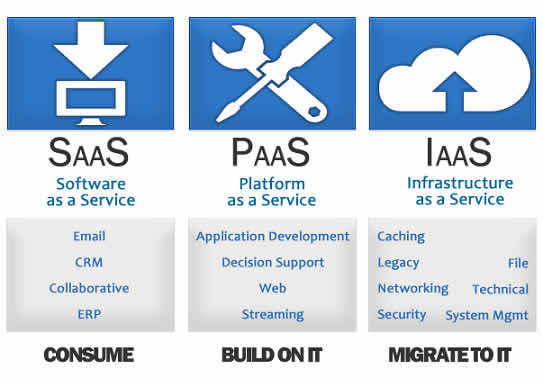
\includegraphics[height=3.5cm, width=4cm]{services}
  \caption{A break down of the main service models.}
  \label{services_figure}
\end{figure}

\subsection{Software as a Service}
Software as a service (SaaS), in which a third party service provider provides the
software.
Cloud application administrations, or Software as a Service (SaaS), portray the biggest
cloud showcase and is evolving rapidly even now. SaaS utilizes the web to convey
applications that are controlled by an outsider seller and whose interface is accessed to
on the customers' side. Most SaaS applications can be run straightforwardly from a web
program with no downloads or installations required, albeit some need the plugins.
On account of the model of web delivery, SaaS eradicates the need to install and run
applications on individual PCs. With SaaS, its simple for business corporations to
streamline their support, on the grounds that everything can be taken care of by the
vendors: applications, runtime, information, middleware, OSes, virtualization, servers,
stockpiling and systems administration.
\subsection{Platform as a Service}
Platform as a service (PaaS), which provides the evolution of newer applications utilizing
the APIs deployed and arranged distantly.
Cloud stage administrations, or Platform as a Service (PaaS), are utilized for applications,
and other innovations, while giving cloud segments to the software. What engineers
pick up with PaaS is a system they can expand upon to create or redo applications. PaaS
makes the testing, improvement, and arrangement of utilizations speedy, basic, and
financially savvy. With this innovation, endeavour operations, or an external supplier,
can oversee OSes, organizing, virtualization, servers, stockpiling, and the PaaS
programming itself. Engineers, on the other hand, deal with the applications.
Undertaking PaaS gives line-of-business programming engineers an organization toward
oneself gateway for overseeing registering framework from brought together IT
operations and the stages that are introduced on top of the equipment. The
undertaking PaaS can be conveyed via a hybrid model that uses both open IaaS and on-
reason framework or as an unadulterated private PaaS that just uses the last.
\subsection{Infrastructure as a Service}
Infrastructure as a service (IaaS), which imparts hardware equipment and the
capabilities of operating systems predominantly through virtualization. Cloud
infrastructure administrations, referred to as Infrastructure as a Service (IaaS), are
organization toward oneself models for getting to, checking, and overseeing remote
datacenter frameworks, for example, register (virtualized or exposed mental),
stockpiling, systems administration (e.g. firewalls). As opposed to needing to buy
equipment out and out, clients can buy IaaS in view of utilization, like power or other
utility charging.
Contrasted with SaaS and PaaS, IaaS clients are in charge of overseeing applications,
information, runtime, middleware, and OSes. Suppliers still oversee virtualization,
servers, hard drives, stockpiling, and systems administration. Numerous IaaS suppliers
now offer databases, informing lines, and different administrations over the
virtualization layer too. Some tech investigators draw a qualification here and utilize the
IaaS+ moniker for these different alternatives. What clients pick up with IaaS is
framework on top of which they can introduce any obliged stage. Clients are in charge
of overhauling these if new forms are discharged.
